\documentclass[a4paper,11pt]{article}
\usepackage[utf8]{inputenc}
\usepackage[russian]{babel}
\usepackage[T1]{fontenc}
\usepackage{amssymb,amsmath,graphicx,indentfirst}
\usepackage{caption}
\usepackage{color}
\usepackage{listings}
\usepackage{enumerate}
\usepackage[unicode]{hyperref}

\setlength{\parskip}{1ex plus 0.5ex minus 0.2ex}
\captionsetup[figure]{labelformat=empty}
\captionsetup[figure]{justification=centering}
\lstset{keywordstyle=\color{blue}\bfseries, basicstyle=\footnotesize}
\lstset{breaklines=true, breakatwhitespace=true}
\lstset{extendedchars=false, language=Caml, defaultdialect=[Objective]Caml}

\author{Олег Смирнов, Александр Полозов \\
\texttt{oleg.smirnov@gmail.com}, \texttt{polozov.alex@gmail.com}}
\date{\today}
\title{Введение в функциональное программирование -- задачи}

\begin{document}
\section*{Модуль 3. Тема 3.1}
\begin{enumerate}[{3-}1]

\item Реализуйте катаморфизм на синтаксическом дереве, который возвращает
  множество переменных, использованных в выражении.
\item Разработайте алгебраический тип и свёртки для следующих задач.

  \begin{enumerate}[(a)]
  \item У нас есть дерево документа, к примеру к лекции 3.1.
  Элементами дерева могут быть:

  \begin{itemize}
  \item параграф
  \item картинка
  \item ссылка
  \item текст
  \end{itemize}
  В каждом параграфе может быть произвольное количество картинок,
  подпараграфов, текста, ссылок и т.д.

  Задача состоит в том, чтобы извлечь все ссылки для того, чтобы вывести
  их в конце презентации. Напишите для этого катаморфизм.

  \item Напишите катаморфизм, который удалит все картинки из документа.
  \end{enumerate}
\end{enumerate}

\section*{Модуль 3. Тема 3.2}

\begin{enumerate}[{3-}1]
  \setcounter{enumi}{2}
\item Реализуйте Rope с размером chunk = 1 (в листьях подвешены единичные
элементы). Балансировка отсутствует. Rope должен быть параметризован тремя
типовыми аргументами: типом данных, хранящихся в дереве, типом меры, и типом
моноида, реализующего операцию над мерой. По-видимому, удобнейший способ это
сделать в отсутствие классов типов -- использовать аналогичную концепцию из
мира ООП, интерфейсы. Заготовка приведена ниже.
\begin{lstlisting}
type IMeasured<'V> = 
    abstract Value : 'V
    
type IMonoid<'V> = 
    abstract Zero : 'V
    abstract Plus : 'V -> 'V -> 'V
    
type Singleton<'T when 'T : (new : unit -> 'T)> private () = 
    static let instance = new 'T()
    static member Instance = instance
    
type Tree<'T, 'M, 'V when 'M :> IMonoid<'V> and 'M : (new : unit -> 'M) and 'T :> IMeasured<'V>> = 
    | Leaf of 'T 
    | Node of 'V * Tree<'T, 'M, 'V> * Tree<'T, 'M, 'V>

type SumMonoid() = 
     interface IMonoid<int> with
         member this.Zero = 0
         member this.Plus a b = a + b
\end{lstlisting}

Здесь приведен интерфейс <<измеримых>> данных, интерфейс моноида, пример
моноида, базовая реализация дерева (обратите внимание, как синтаксис F\#
позволяет наложить дополнительные ограничения на типовые параметры).
Оператор \texttt{:>} значит <<является подтипом>>.

Отдельное внимание обратите на синглтон. Это известный паттерн в промышленном
программировании: тип, у которого одновременно может существовать только один
экземпляр. Это именно то, что нам нужно, чтобы пользоваться моноидами:
моноидальная операция \texttt{Plus} принадлежит типу, а не его экземплярам,
но для её вызовов экземпляры все-таки приходится создавать. Чтобы избавиться
от этого неудобства, тип моноида делают синглтоном. Тогда, чтобы обращаться к
операции, можно использовать следующий код:
\begin{lstlisting}
let monoid = Singleton<SumMonoid>.Instance
let x = monoid.Plus l r
\end{lstlisting}

\begin{enumerate}
\item Для этого Rope реализуйте:
\begin{itemize}
\item Построение дерева по массиву (списку) данных, произвольным способом.
Желательно организовать построение так, чтобы полученное дерево сразу имело
высоту $O(\log N)$.
\item Изменение элемента по индексу (с перевычислением мер по пути).
\item Слияние двух веревок за $O(1)$.
\item Вычисление меры на подотрезке.
\item Разрезание по предикату.
\end{itemize}
Если какие-то из операций удастся реализовать через уже реализованные другие
-- отлично, это только лучше.
\item Реализуйте моноид статических характеристик выборки. Пользуясь классом
\texttt{System.Random}, сгенерируйте 100 выборок размера 50, постройте из них
дерево и выведите характеристики результирующей выборки. Проверьте результат,
слив выборки вручную и подсчитав характеристики по определению.

\item \textbf{*} Имеется кабель из $k$ проводов, который идет из точки $A$ в
точку $B$. Кабель выходит на поверхность в $N$ местах, не считая начало и конец
($N \le 10^5$). Между этими точками кабель залегает глубоко под землей, и
доступа к нему нет.

У монтера-электрика дяди Васи выдался плохой день, и этим вечером он,
основательно отдохнув, решил отомстить всему этому несправедливому миру. На
протяжении вечера во время <<основательного отдыха>> периодически дядя Вася
озлобляется и идет к кабелю -- мстить за свой плохой день. Всего за день это
произошло $T$ раз ($T \le 10^5$).

Суть каждой мести заключается в том, что дядя Вася идет к какому-нибудь из
$N$ мест, откуда он может достать до кабеля, разрезает его и перепутывает в
нем провода. Более строго, дядя Вася выбирает какое-то место $1\le i\le N$ и
разрезает кабель в этом месте. Теперь в левой руке (ближней к точке $A$) у
него $k$ проводов в ряд, и в правой руке (ближней к точке $B$) у него тоже
$k$ проводов в ряд. Дядя Вася каким-то случайным образом присоединяет каждый
из $k$ проводов слева к какому-то из $k$ проводов справа (взаимно однозначно),
заматывает все изолентой и со злорадной улыбкой удаляется. Теперь информация,
посланная из точки $A$ по проводу №$j$ ($1\le j \le k$), придет в точку $B$
не на выход №$j$, а на какой-то другой.

Поскольку всю эту процедуру дядя Вася проделывал $T$ раз в разных местах
кабеля, все провода безнадежно перепутались. Наутро неблагодарные жильцы
района нашли дядю Васю и убедительно попросили его рассказать им, какой же
из выходов кабеля какому входу теперь соответствует. После продуктивного
вечернего отдыха дядя Вася оказался не в силах решить такую тяжелую
вычислительную задачу. Зато, к своему удивлению, он помнил в точности, какие
локальные перепутывания в каких точках он производил. То есть, для каждого из
$T$ перепутываний в хронологическом порядке дядя Вася может рассказать, какие
провода в левой руке он соединял с какими проводами в правой руке, а также где
это все происходило. Естественно, что, поскольку перепутываний было много, то
провод №1 в левой руке дяди Васи к концу вечера совершенно не обязательно
соответствует проводу №1 в точке $A$. С правой рукой та же проблема.

Вам дан список $T$ воспоминаний дяди Васи. Каждое воспоминание содержит точку
очередной диверсии $n$ ($1 \le n \le N$) и список соответствий перепутывания в
нумерации с точки зрения дяди Васи, глядящего в этот момент на разрезанный
кабель (например, $1 \to 5, 2 \to 3, 3 \to 8, \ldots$). Гарантируется, что
воспоминания даны в хронологическом порядке.

Пользуясь теорией моноидальных вычислений и запрограммированным ранее деревом,
помогите жильцам района и вычислите итоговую таблицу соответствия проводов
кабеля в точке $A$ проводам в точке $B$ после всех махинаций дяди Васи.

К примеру, пусть $k=4$, $N=3$, $T=2$. Первое перепутывание происходит в точке
$n=3$ по схеме $1\to2,2\to4,3\to3,4\to1$, второе -- в точке $n=1$ по схеме
$1\to2,2\to4,3\to1,4\to3$. Тогда в итоге провода будут соответствовать 
следующим образом: $1\to4,2\to1,3\to2,4\to3$ (см. рисунок).
\begin{center}
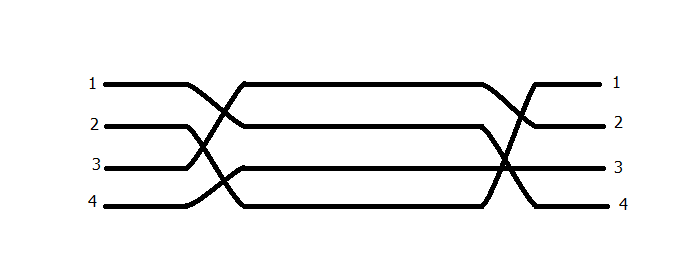
\includegraphics[scale=0.6]{problems2/wires.png}
\end{center}
\end{enumerate}
\end{enumerate}
\end{document}
